\section{Can relationship use survive a change of world?}
\label{sec:transfer}

Finetuning may teach evidence use or merely typical answers. We test whether
training transfers relationships to new worlds and improves unseen-event forecasts.

\subsection{Exp.~3: what training transfers, and what it does not}
\label{sec:exp3}

% Generated by exp3_training_transfer/render_exp3_paper_macros.py
% Do not edit. Every Experiment 3 number in the prose comes from here.
\providecommand{\eEightBaseParse}{99.83}
\providecommand{\eEightDomainBaseGainCi}{[5.266,5.454]}
\providecommand{\eEightDomainBaseGainParsedCi}{[5.266,5.454]}
\providecommand{\eEightDomainBaseGainParsed}{5.360}
\providecommand{\eEightDomainBaseGain}{5.360}
\providecommand{\eEightDomainBase}{7.30}
\providecommand{\eEightDomainCi}{[-.026,.269]}
\providecommand{\eEightDomainEst}{.110}
\providecommand{\eEightDomainMatched}{1.89}
\providecommand{\eEightDomainPrior}{2.00}
\providecommand{\eEightDomainSignP}{.1445}
\providecommand{\eEightDomainSign}{6/8}
\providecommand{\eEightDomainTci}{[-.072,.292]}
\providecommand{\eEightDomainWild}{.1772}
\providecommand{\eEightG}{8}
\providecommand{\eEightIdBaseGainCi}{[3.437,3.481]}
\providecommand{\eEightIdBaseGainParsedCi}{[3.119,3.163]}
\providecommand{\eEightIdBaseGainParsed}{3.141}
\providecommand{\eEightIdBaseGain}{3.459}
\providecommand{\eEightIdBase}{3.96}
\providecommand{\eEightIdCi}{[.018,.112]}
\providecommand{\eEightIdEst}{.060}
\providecommand{\eEightIdMatched}{.47}
\providecommand{\eEightIdPrior}{.53}
\providecommand{\eEightIdSignP}{.0039}
\providecommand{\eEightIdSign}{8/8}
\providecommand{\eEightIdTci}{[.005,.115]}
\providecommand{\eEightIdWild}{.0089}
\providecommand{\eEightJointBaseGainCi}{[1.063,1.196]}
\providecommand{\eEightJointBaseGainParsedCi}{[.611,.744]}
\providecommand{\eEightJointBaseGainParsed}{.677}
\providecommand{\eEightJointBaseGain}{1.129}
\providecommand{\eEightJointBase}{5.72}
\providecommand{\eEightJointCi}{[-.002,.265]}
\providecommand{\eEightJointEst}{.126}
\providecommand{\eEightJointMatched}{4.53}
\providecommand{\eEightJointPrior}{4.65}
\providecommand{\eEightJointSignP}{.1445}
\providecommand{\eEightJointSign}{6/8}
\providecommand{\eEightJointTci}{[-.035,.287]}
\providecommand{\eEightJointWild}{.0906}
\providecommand{\eEightStructureBaseGainCi}{[-.051,-.023]}
\providecommand{\eEightStructureBaseGainParsedCi}{[-.051,-.023]}
\providecommand{\eEightStructureBaseGainParsed}{-.037}
\providecommand{\eEightStructureBaseGain}{-.037}
\providecommand{\eEightStructureBase}{2.30}
\providecommand{\eEightStructureCi}{[-.056,.040]}
\providecommand{\eEightStructureEst}{-.003}
\providecommand{\eEightStructureMatched}{2.34}
\providecommand{\eEightStructurePrior}{2.34}
\providecommand{\eEightStructureSignP}{.1445}
\providecommand{\eEightStructureSign}{6/8}
\providecommand{\eEightStructureTci}{[-.057,.051]}
\providecommand{\eEightStructureWild}{.9177}
\providecommand{\eFourbBaseParse}{99.97}
\providecommand{\eFourbDomainBaseGainCi}{[6.581,6.802]}
\providecommand{\eFourbDomainBaseGainParsedCi}{[6.581,6.802]}
\providecommand{\eFourbDomainBaseGainParsed}{6.692}
\providecommand{\eFourbDomainBaseGain}{6.692}
\providecommand{\eFourbDomainBase}{8.53}
\providecommand{\eFourbDomainCi}{[-.091,.255]}
\providecommand{\eFourbDomainEst}{.087}
\providecommand{\eFourbDomainMatched}{1.80}
\providecommand{\eFourbDomainPrior}{1.88}
\providecommand{\eFourbDomainSignP}{.3633}
\providecommand{\eFourbDomainSign}{5/8}
\providecommand{\eFourbDomainTci}{[-.130,.303]}
\providecommand{\eFourbDomainWild}{.3569}
\providecommand{\eFourbG}{8}
\providecommand{\eFourbIdBaseGainCi}{[3.075,3.166]}
\providecommand{\eFourbIdBaseGainParsedCi}{[3.075,3.166]}
\providecommand{\eFourbIdBaseGainParsed}{3.121}
\providecommand{\eFourbIdBaseGain}{3.121}
\providecommand{\eFourbIdBase}{3.82}
\providecommand{\eFourbIdCi}{[-.056,.194]}
\providecommand{\eFourbIdEst}{.067}
\providecommand{\eFourbIdMatched}{.67}
\providecommand{\eFourbIdPrior}{.74}
\providecommand{\eFourbIdSignP}{.6367}
\providecommand{\eFourbIdSign}{4/8}
\providecommand{\eFourbIdTci}{[-.091,.225]}
\providecommand{\eFourbIdWild}{.3444}
\providecommand{\eFourbJointBaseGainCi}{[1.362,1.551]}
\providecommand{\eFourbJointBaseGainParsedCi}{[1.362,1.551]}
\providecommand{\eFourbJointBaseGainParsed}{1.457}
\providecommand{\eFourbJointBaseGain}{1.457}
\providecommand{\eFourbJointBase}{6.15}
\providecommand{\eFourbJointCi}{[-.032,.298]}
\providecommand{\eFourbJointEst}{.136}
\providecommand{\eFourbJointMatched}{4.63}
\providecommand{\eFourbJointPrior}{4.76}
\providecommand{\eFourbJointSignP}{.1445}
\providecommand{\eFourbJointSign}{6/8}
\providecommand{\eFourbJointTci}{[-.072,.344]}
\providecommand{\eFourbJointWild}{.1583}
\providecommand{\eFourbStructureBaseGainCi}{[.153,.275]}
\providecommand{\eFourbStructureBaseGainParsedCi}{[.153,.275]}
\providecommand{\eFourbStructureBaseGainParsed}{.214}
\providecommand{\eFourbStructureBaseGain}{.214}
\providecommand{\eFourbStructureBase}{2.66}
\providecommand{\eFourbStructureCi}{[-.075,.179]}
\providecommand{\eFourbStructureEst}{.052}
\providecommand{\eFourbStructureMatched}{2.43}
\providecommand{\eFourbStructurePrior}{2.48}
\providecommand{\eFourbStructureSignP}{.3633}
\providecommand{\eFourbStructureSign}{5/8}
\providecommand{\eFourbStructureTci}{[-.110,.214]}
\providecommand{\eFourbStructureWild}{.4623}
\providecommand{\eMechDiscCi}{[.278,.404]}
\providecommand{\eMechDiscEst}{.337}
\providecommand{\eMechDiscSd}{.073}
\providecommand{\eMechDiscSignP}{.0312}
\providecommand{\eMechDiscSign}{5/5}
\providecommand{\eMechDiscTci}{[.247,.428]}
\providecommand{\eMechDiscWild}{.0130}
\providecommand{\eMechG}{5}
\providecommand{\eMechUndiscCi}{[.328,.387]}
\providecommand{\eMechUndiscEst}{.357}
\providecommand{\eMechUndiscSd}{.033}
\providecommand{\eMechUndiscSignP}{.0312}
\providecommand{\eMechUndiscSign}{5/5}
\providecommand{\eMechUndiscTci}{[.316,.399]}
\providecommand{\eMechUndiscWild}{.0021}
\providecommand{\ePubEightDomainCi}{[.026,.545]}
\providecommand{\ePubEightDomainEst}{.241}
\providecommand{\ePubEightIdCi}{[.002,.187]}
\providecommand{\ePubEightIdEst}{.081}
\providecommand{\ePubEightJointCi}{[.058,.470]}
\providecommand{\ePubEightJointEst}{.251}
\providecommand{\ePubEightStructureCi}{[-.011,.071]}
\providecommand{\ePubEightStructureEst}{.029}
\providecommand{\ePubFourbDomainCi}{[.039,.383]}
\providecommand{\ePubFourbDomainEst}{.230}
\providecommand{\ePubFourbIdCi}{[.112,.319]}
\providecommand{\ePubFourbIdEst}{.209}
\providecommand{\ePubFourbJointCi}{[.134,.489]}
\providecommand{\ePubFourbJointEst}{.319}
\providecommand{\ePubFourbStructureCi}{[.023,.353]}
\providecommand{\ePubFourbStructureEst}{.190}
\providecommand{\ePubLlamaDomainCi}{[-.868,-.243]}
\providecommand{\ePubLlamaDomainEst}{-.581}
\providecommand{\ePubLlamaIdCi}{[-.680,-.130]}
\providecommand{\ePubLlamaIdEst}{-.351}
\providecommand{\ePubLlamaJointCi}{[-.115,.958]}
\providecommand{\ePubLlamaJointEst}{.420}
\providecommand{\ePubLlamaStructureCi}{[-.862,.306]}
\providecommand{\ePubLlamaStructureEst}{-.167}
\providecommand{\eSelBasePersistDir}{1.19}
\providecommand{\eSelBasePersistMed}{1.21}
\providecommand{\eSelCityArbBase}{-.005}
\providecommand{\eSelCityArbCi}{[-.012,.001]}
\providecommand{\eSelCityArbEst}{-.005}
\providecommand{\eSelCitySemBase}{.020}
\providecommand{\eSelCitySemCi}{[-.011,.019]}
\providecommand{\eSelCitySemEst}{.004}
\providecommand{\eSelHarborArbBase}{.002}
\providecommand{\eSelHarborArbCi}{[-.016,.009]}
\providecommand{\eSelHarborArbEst}{-.004}
\providecommand{\eSelHarborSemBase}{.068}
\providecommand{\eSelHarborSemCi}{[-.023,.022]}
\providecommand{\eSelHarborSemEst}{-.001}
\providecommand{\eSelTrainedPersistHi}{.59}
\providecommand{\eSelTrainedPersistLo}{.49}

\newcommand{\transfergridlines}{15}
% Compact inline orientation graphic for the Experiment 3 transfer design: a 2x2
% grid crossing generative mechanism (rows) with surface domain (columns).
%
% Row cards carry the mechanism detail: a two-node vs three-node graph with the
% mediator drawn hollow (it is never named to the model) and a persistence loop,
% plus the six-period impulse response on labelled axes. Bar heights are the
% normalised responses to a unit shock under worlds.transition at the midpoint of
% each sampling band (direct: gain .57; mediated: gain .57, rho .61, phi .30,
% lambda .81), i.e. A = (1, 0, 0, 0, 0, 0) and B = (.81, .74, .52, .34, .21, .13).
%
% Geometry note: cards have fixed dimensions and every label is a single line
% with no text width, so nothing can rewrap into a neighbour.
% Callers may set \transfergridlines to match the paragraph they anchor this
% to; wrapfig cannot wrap a section heading, so the count must not overrun it.
\providecommand{\transfergridlines}{13}
\begin{wrapfigure}[\transfergridlines]{r}{0.48\textwidth}
\vspace{-0.8em}
\centering
\definecolor{miniCityFill}{HTML}{E8F2FB}
\definecolor{miniCityEdge}{HTML}{4F7EA8}
\definecolor{miniHarborEdge}{HTML}{3F8E82}
\definecolor{miniTestFill}{HTML}{E7F4EA}
\definecolor{miniTestEdge}{HTML}{6FA97F}
\definecolor{miniTestChip}{HTML}{5E9470}
% Coin discs reuse Figure 1's yellow pair exactly -- the fill and stroke of its
% NAIVE box -- rather than the saturated gold used before. Figure 1's other warm
% pair (#FFE6CC on #D79B00, its FREQUENTIST box) is the orange one and is not
% used here. The glyph inside each disc still carries its domain colour.
\definecolor{miniCoinFill}{HTML}{FFF2CC}
\definecolor{miniCoinRim}{HTML}{D6B656}
\definecolor{miniMute}{HTML}{8A93A3}
\definecolor{miniInk}{HTML}{3F4550}
\definecolor{miniBar}{HTML}{7C93AD}
% Coin City: a skyline stamped into a coin.
\newcommand{\coincity}[2]{%
  \begin{scope}[shift={(#1,#2)},scale=0.70]
    \fill[miniCoinFill] (0,0) circle (.37);
    \draw[miniCoinRim,line width=.75pt] (0,0) circle (.37);
    \fill[miniCityEdge] (-.23,-.18) rectangle (-.10,.04);
    \fill[miniCityEdge] (-.07,-.18) rectangle (.07,.16);
    \fill[miniCityEdge] (.10,-.18) rectangle (.24,.09);
    \draw[miniCityEdge,line width=.65pt] (-.27,-.19)--(.27,-.19);
  \end{scope}}
% Coin Harbor: a small vessel and waves stamped into a coin.
\newcommand{\coinharbor}[2]{%
  \begin{scope}[shift={(#1,#2)},scale=0.70]
    \fill[miniCoinFill] (0,0) circle (.37);
    \draw[miniCoinRim,line width=.75pt] (0,0) circle (.37);
    \fill[miniHarborEdge] (-.24,-.05)--(.24,-.05)--(.15,-.18)--(-.15,-.18)--cycle;
    \draw[miniHarborEdge,line width=.7pt]
      (-.01,-.05)--(-.01,.15)--(.15,.02)--(-.01,.02);
    \draw[miniHarborEdge,line width=.55pt]
      (-.26,-.24)..controls(-.18,-.19)and(-.10,-.29)..(-.02,-.24)
      ..controls(.06,-.19)and(.14,-.29)..(.26,-.24);
  \end{scope}}
% Impulse response on labelled axes: response (Delta y) against period (t).
\newcommand{\impulse}[3]{% #1 = axis corner x, #2 = baseline y, #3 = bar heights
  \draw[-{Stealth[length=2.6pt,width=2.2pt]},draw=miniInk!65,line width=.5pt]
    (#1,#2) -- (#1,#2+0.40);
  \draw[-{Stealth[length=2.6pt,width=2.2pt]},draw=miniInk!65,line width=.5pt]
    (#1,#2) -- (#1+0.72,#2);
  \node[anchor=south,font=\sffamily\scriptsize,text=miniInk,inner sep=1pt]
    at (#1,#2+0.40) {$\Delta y$};
  \node[anchor=west,font=\sffamily\scriptsize,text=miniInk,inner sep=1.5pt]
    at (#1+0.72,#2) {$t$};
  \foreach \i/\h in {#3}{%
    \fill[miniBar] (#1+0.055+\i*0.105,#2) rectangle (#1+0.055+\i*0.105+0.070,#2+\h);}}
\resizebox{\linewidth}{!}{%
\begin{tikzpicture}[
  x=1cm, y=1cm,
  cell/.style={rounded corners=3pt, minimum width=1.95cm, minimum height=1.25cm,
    line width=.6pt, inner sep=0pt},
  traincell/.style={cell, draw=miniCityEdge, fill=miniCityFill},
  heldcell/.style={cell, draw=miniTestEdge, fill=miniTestFill,
    dash pattern=on 1.9pt off 1.5pt},
  rowcard/.style={rounded corners=3pt, minimum width=2.60cm,
    minimum height=1.25cm, inner sep=0pt, draw=miniMute!30, fill=black!3,
    line width=.5pt},
  dname/.style={anchor=south, font=\sffamily\bfseries\scriptsize},
  rname/.style={anchor=center, font=\sffamily\scriptsize, text=miniInk},
  note/.style={anchor=center, font=\sffamily\scriptsize, text=miniInk},
  gnode/.style={circle, draw=miniInk!75, fill=white, line width=.5pt,
    inner sep=0pt, minimum size=0.26cm, font=\sffamily\tiny, text=miniInk},
  hidden/.style={gnode, draw=miniMute, fill=miniMute!14,
    dash pattern=on 1.1pt off .9pt},
  garrow/.style={-{Stealth[length=2.4pt,width=2pt]}, draw=miniInk!70,
    line width=.45pt, shorten >=.4pt, shorten <=.4pt},
  chip/.style={anchor=center, rounded corners=1.6pt, draw=none, text=white,
    inner xsep=3pt, inner ysep=1.1pt, font=\sffamily\bfseries\tiny},
]
% ---- domain marks and names ----------------------------------------------
\coincity{0.975}{2.56}
\coinharbor{3.075}{2.56}
\node[dname, text=miniCityEdge]   at (0.975,1.80) {COIN CITY};
\node[dname, text=miniHarborEdge] at (3.075,1.80) {COIN HARBOR};

% ---- Structure A: direct, one period -------------------------------------
\node[rowcard] at (-1.50,1.00) {};
\node[rname] at (-1.50,1.45) {\textbf{Structure A} direct};
\node[gnode] (ax) at (-2.51,0.82) {$x$};
\node[gnode] (ay) at (-2.07,0.82) {$y$};
\draw[garrow] (ax) -- (ay);
\impulse{-1.22}{0.62}{0/0.360, 1/0.000, 2/0.000, 3/0.000, 4/0.000, 5/0.000}

% ---- Structure B: mediated, persistent -----------------------------------
\node[rowcard] at (-1.50,-0.42) {};
\node[rname] at (-1.50,0.03) {\textbf{Structure B} mediated};
\node[gnode]  (bx) at (-2.51,-0.60) {$x$};
\node[hidden] (bm) at (-2.07,-0.60) {$m$};
\node[gnode]  (by) at (-1.63,-0.60) {$y$};
\draw[garrow] (bx) -- (bm);
\draw[garrow] (bm) -- (by);
\draw[garrow] (bm) to[out=118,in=62,looseness=4.5] (bm);
\impulse{-1.22}{-0.80}{0/0.292, 1/0.265, 2/0.188, 3/0.123, 4/0.077, 5/0.048}

% ---- the four evaluation cells -------------------------------------------
\node[traincell] at (0.975,1.00) {};
\node[heldcell]  at (3.075,1.00) {};
\node[heldcell]  at (0.975,-0.42) {};
\node[heldcell]  at (3.075,-0.42) {};

\node[chip, fill=miniCityEdge] at (0.975,1.26) {TRAINED};
\node[chip, fill=miniTestChip] at (3.075,1.26) {TEST};
\node[chip, fill=miniTestChip] at (0.975,-0.16) {TEST};
\node[chip, fill=miniTestChip] at (3.075,-0.16) {TEST};

\node[note] at (0.975,0.80) {in-distribution};
\node[note] at (3.075,0.80) {domain shift};
\node[note] at (0.975,-0.62) {structure shift};
\node[note] at (3.075,-0.62) {joint shift};
\end{tikzpicture}%
}
\vspace{-0.3em}
\caption{\textbf{Transfer grid.} Training uses shading;
all four are evaluated. Columns vary domain; rows vary response mechanism.}
\label{fig:exp3-transfer-grid}
\vspace{0.1em}
\end{wrapfigure}


\textbf{Why matching matters.}
The parent experiment compares byte-identical prompts, identical target-answer
multisets, and equal training budgets, changing only case--answer pairing.
Figure~\ref{fig:exp3-transfer-grid} crosses a domain change---campaign news and
candidate support become shipping bulletins and cargo flow---with a change
from direct to persistent responses (App.~\ref{app:exp3-complete-training-setup}).

\noindent\textbf{Finding: domain transfer is stronger than structural transfer.}
Training generalizes across the surface change. Across both arms and
\eEightG{} seeds, Qwen3-8B reduces domain-shift response error by
\eEightDomainBaseGain{} points \eEightDomainBaseGainCi{}, with every seed agreeing.
The matched arm reaches \eEightDomainMatched{} versus the base's
\eEightDomainBase{}.
Because unparsed draws take the full
range penalty, we report base contrasts twice: the joint-cell gain is
\eEightJointBaseGain{} \eEightJointBaseGainCi{} fail-closed and
\eEightJointBaseGainParsed{} \eEightJointBaseGainParsedCi{} on parsed draws.

% Experiment 3 transfer results, laid out on the same 2x2 grid as the design
% figure (Figure~\ref{fig:exp3-transfer-grid}) so the reader reads results in the
% cells they were introduced in: mechanism down the rows, surface domain across
% the columns, the trained cell shaded blue and the three held-out cells green.
%
% Every number comes from tables/exp3_coin_qwen3_8b_stochastic_data.tex,
% regenerated by coin_city_structural/make_qwen3_8b_eight_seed_outputs.py. Bar
% lengths share one scale
% (\cciPeak) across all four cells so cells are comparable by eye. Do not put
% formatting logic here: emphasis on an interval that excludes zero is decided
% by the generator and arrives pre-set in \cci*delta.
% generated by coin_city_structural/make_qwen3_8b_eight_seed_outputs.py (90% bootstrap percentile bounds) -- do not edit
% G=8 seeds [42, 43, 44, 45, 46, 47, 48, 49]
% Bold marks a 90% interval (5th, 95th bootstrap percentiles) excluding zero;
% 2 of 4 cells qualify at 90%.
\newcommand{\cciPeak}{7.30}
\newcommand{\cciIDbase}{3.96}
\newcommand{\cciIDprior}{0.53}
\newcommand{\cciIDmatched}{0.47}
\newcommand{\cciIDdelta}{\textbf{0.06} [0.02, 0.10]}
\newcommand{\cciDomainbase}{7.30}
\newcommand{\cciDomainprior}{2.00}
\newcommand{\cciDomainmatched}{1.89}
\newcommand{\cciDomaindelta}{0.11 [-0.01, 0.24]}
\newcommand{\cciStructurebase}{2.30}
\newcommand{\cciStructureprior}{2.34}
\newcommand{\cciStructurematched}{2.34}
\newcommand{\cciStructuredelta}{-0.00 [-0.05, 0.03]}
\newcommand{\cciJointbase}{5.72}
\newcommand{\cciJointprior}{4.65}
\newcommand{\cciJointmatched}{4.53}
\newcommand{\cciJointdelta}{\textbf{0.13} [0.02, 0.24]}

\begin{figure}[!ht]
\centering
\definecolor{gCityFill}{HTML}{E8F2FB}
\definecolor{gCityEdge}{HTML}{4F7EA8}
\definecolor{gHarborEdge}{HTML}{3F8E82}
\definecolor{gTestFill}{HTML}{E7F4EA}
\definecolor{gTestEdge}{HTML}{6FA97F}
\definecolor{gTestChip}{HTML}{5E9470}
\definecolor{gCoinFill}{HTML}{FFF2CC}
\definecolor{gCoinRim}{HTML}{D6B656}
\definecolor{gInk}{HTML}{3F4550}
\definecolor{gMute}{HTML}{8A93A3}
\definecolor{gBarBase}{HTML}{C3CBD4}
\definecolor{gBarLess}{HTML}{A9B4C0}
\definecolor{gBarPrior}{HTML}{7C93AD}
\definecolor{gBarMatched}{HTML}{4F7EA8}
\newcommand{\gcoincity}[2]{%
  \begin{scope}[shift={(#1,#2)},scale=0.70]
    \fill[gCoinFill] (0,0) circle (.37);
    \draw[gCoinRim,line width=.75pt] (0,0) circle (.37);
    \fill[gCityEdge] (-.23,-.18) rectangle (-.10,.04);
    \fill[gCityEdge] (-.07,-.18) rectangle (.07,.16);
    \fill[gCityEdge] (.10,-.18) rectangle (.24,.09);
    \draw[gCityEdge,line width=.65pt] (-.27,-.19)--(.27,-.19);
  \end{scope}}
\newcommand{\gcoinharbor}[2]{%
  \begin{scope}[shift={(#1,#2)},scale=0.70]
    \fill[gCoinFill] (0,0) circle (.37);
    \draw[gCoinRim,line width=.75pt] (0,0) circle (.37);
    \fill[gHarborEdge] (-.24,-.05)--(.24,-.05)--(.15,-.18)--(-.15,-.18)--cycle;
    \draw[gHarborEdge,line width=.7pt] (-.01,-.05)--(-.01,.15)--(.15,.02)--(-.01,.02);
    \draw[gHarborEdge,line width=.55pt]
      (-.26,-.24)..controls(-.18,-.19)and(-.10,-.29)..(-.02,-.24)
      ..controls(.06,-.19)and(.14,-.29)..(.26,-.24);
  \end{scope}}
% One results card. #1 cx, #2 cy, #3 cell name, #4 chip text, #5 chip fill,
% #6..#8 base/prior/episode-matched MAE; the contrast is placed separately.
\newcommand{\gcard}[8]{%
  \node[cellname] at (#1-2.66,#2+0.78) {#3};
  \node[chip, fill=#5] at (#1+2.66,#2+0.78) {#4};
  \foreach \arm/\val/\col/\dy in {%
      base/#6/gBarBase/0.34, prior/#7/gBarPrior/0.00,
      episode-matched/#8/gBarMatched/-0.34}{%
    \node[armlab] at (#1-2.66,#2+\dy) {\arm};
    \fill[\col, rounded corners=1pt]
      (#1-0.55,#2+\dy-0.075) rectangle (#1-0.55+\val*2.55/\cciPeak,#2+\dy+0.075);
    \node[armval] at (#1-0.43+\val*2.55/\cciPeak,#2+\dy) {\val};}}
\resizebox{.96\linewidth}{!}{%
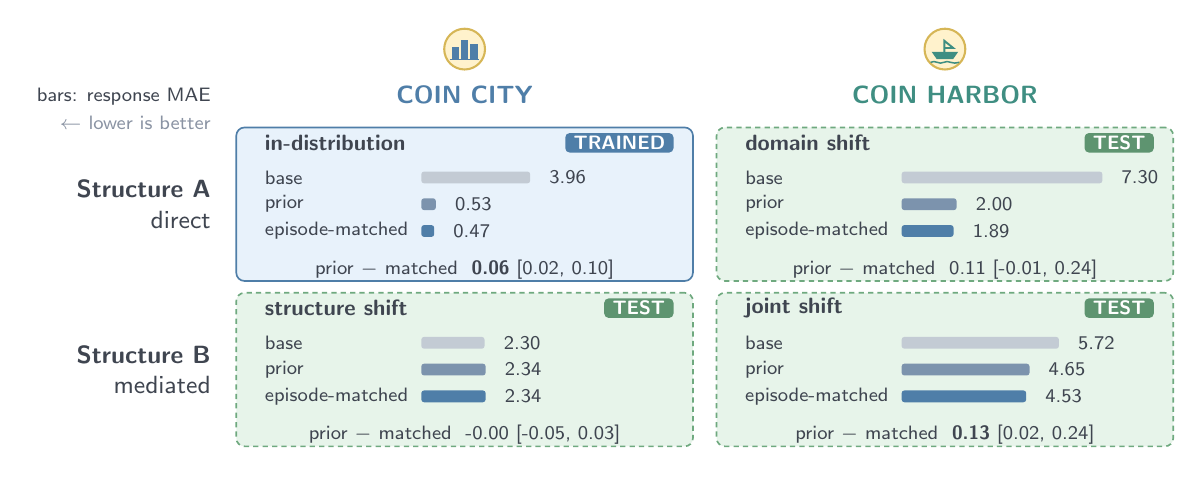
\begin{tikzpicture}[
  x=1cm, y=1cm,
  card/.style={rounded corners=3pt, minimum width=5.80cm, minimum height=1.95cm,
    line width=.6pt, inner sep=0pt},
  traincard/.style={card, draw=gCityEdge, fill=gCityFill},
  testcard/.style={card, draw=gTestEdge, fill=gTestFill,
    dash pattern=on 1.9pt off 1.5pt},
  dname/.style={anchor=south, font=\sffamily\bfseries\small},
  rname/.style={anchor=east, align=right, font=\sffamily\small, text=gInk},
  cellname/.style={anchor=west, font=\sffamily\bfseries\footnotesize, text=gInk},
  chip/.style={anchor=east, rounded corners=1.6pt, draw=none, text=white,
    inner xsep=3pt, inner ysep=1.1pt, font=\sffamily\bfseries\scriptsize},
  armlab/.style={anchor=west, font=\sffamily\scriptsize, text=gInk},
  armval/.style={anchor=west, font=\sffamily\scriptsize, text=gInk},
  delta/.style={anchor=center, font=\sffamily\scriptsize, text=gInk},
  legend/.style={anchor=east, font=\sffamily\scriptsize},
]
% ---- domain columns ------------------------------------------------------
\gcoincity{2.90}{3.22}
\gcoinharbor{9.00}{3.22}
\node[dname, text=gCityEdge]   at (2.90,2.40) {COIN CITY};
\node[dname, text=gHarborEdge] at (9.00,2.40) {COIN HARBOR};

% ---- what the bars mean, and which way is good --------------------------
\node[legend, text=gInk]  at (-0.20,2.62) {bars: response MAE};
\node[legend, text=gMute] at (-0.20,2.28) {$\leftarrow$ lower is better};

% ---- mechanism rows ------------------------------------------------------
\node[rname] at (-0.20,1.25) {\textbf{Structure A}\\ direct};
\node[rname] at (-0.20,-0.85) {\textbf{Structure B}\\ mediated};

% ---- the four result cards ----------------------------------------------
\node[traincard] at (2.90,1.25) {};
\node[testcard]  at (9.00,1.25) {};
\node[testcard]  at (2.90,-0.85) {};
\node[testcard]  at (9.00,-0.85) {};

\gcard{2.90}{1.25}{in-distribution}{TRAINED}{gCityEdge}
  {\cciIDbase}{\cciIDprior}{\cciIDmatched}
\node[delta] at (2.90,0.42) {prior $-$ matched\ \ \cciIDdelta};

\gcard{9.00}{1.25}{domain shift}{TEST}{gTestChip}
  {\cciDomainbase}{\cciDomainprior}{\cciDomainmatched}
\node[delta] at (9.00,0.42) {prior $-$ matched\ \ \cciDomaindelta};

\gcard{2.90}{-0.85}{structure shift}{TEST}{gTestChip}
  {\cciStructurebase}{\cciStructureprior}{\cciStructurematched}
\node[delta] at (2.90,-1.68) {prior $-$ matched\ \ \cciStructuredelta};

\gcard{9.00}{-0.85}{joint shift}{TEST}{gTestChip}
  {\cciJointbase}{\cciJointprior}{\cciJointmatched}
\node[delta] at (9.00,-1.68) {prior $-$ matched\ \ \cciJointdelta};
\end{tikzpicture}%
}
\caption{\textbf{Qwen3-8B Coin City transfer at round 300 under five-draw
stochastic decoding, eight training seeds.} Bars show task-averaged response MAE
over four evidence depths; trained arms average eight seeds. Each cell prints the
paired seed-first prior-minus-matched contrast, bold when its 95\% interval
excludes zero. At three seeds three of the four contrasts excluded zero; at eight
only the in-distribution cell does. The structure-shift row is a control rather than
a transfer test: training contains no structural variation, so the trained policy
emits no delayed response anywhere (Section~\ref{sec:exp3}).}
\label{fig:exp3-transfer-results}
\vspace{10pt}
\end{figure}


The finer contrast between episode-matched and shuffled-pair training does not
survive replication. Estimated at three seeds and extended to eight under a
pre-registered amendment, the Qwen3-8B joint-shift contrast falls from
\ePubEightJointEst{} \ePubEightJointCi{} to \eEightJointEst{} \eEightJointCi{};
all four of Qwen3-4B's cells excluded zero at three seeds and all span it at
eight. A wrapper crossover retains a similar three-seed mean ($.251$ versus $.255$;
App.~\ref{app:exp3-eight-seed}). One cell survives every test: Qwen3-8B in distribution,
\eEightIdEst{} \eEightIdCi{}, \eEightIdSign{} seeds, clearing the conservative
$t$ \eEightIdTci{}, a wild cluster bootstrap ($p=\eEightIdWild{}$) and an exact
sign test ($p=\eEightIdSignP{}$). It does not replicate on Qwen3-4B, and
Llama-3.1-8B's estimate has the opposite sign.

\noindent\textbf{Response-form selection is learnable, but transfer is limited.}
The original structure-shift row is a control: training contains only the direct
response, and every trained checkpoint emits zero delayed response. We therefore
rebuilt the task with both forms in training: two references have identical
horizon-1 responses but differ in persistence, and a cue names which the target
follows. Three-seed Qwen3-8B RL learns marginal persistence without reliable cue
following (App.~\ref{app:exp3-structure-selection}).

In a fixed component diagnostic crossing both domains and semantic or arbitrary
labels, all eight checkpoints identify the named reference perfectly.
Supplying exact response patterns does not rescue the 8B forecasts; an untrained
32B model shows partial numerical ability but often omits the resting baseline
(App.~\ref{app:exp3-components}). An exploratory, single-seed supervised pilot on the same
4,800 training prompts yields $97.9\%$ forecast structure accuracy in Coin City/semantic,
versus $50.0\%$ for matched RL. It falls to $39.6\%$
with arbitrary labels and $45.8\%$/$50.0\%$ in Coin Harbor with semantic/arbitrary
labels. The lower-rate supervised recipe reaches only $58.3\%$ in distribution.
Learning rate and update budget differ, limiting this to in-domain learnability
under one recipe, not a general SFT advantage or transferable induction (App.~\ref{app:exp3-learnability}).

\noindent\textbf{Composition accuracy and evidence use are distinct.}
On the mechanism-family benchmark, episode-matched Qwen3-4B training beats a
\emph{fixed population-prior} control on held-out compositions: response-MAE
advantages are \eMechDiscEst{} \eMechDiscCi{} with the mechanism described and
\eMechUndiscEst{} \eMechUndiscCi{} with it inferred, both clearing all four
estimators at \eMechG{} seeds. A coherent gain intervention with two retained checkpoint seeds shows better
tracking than the prior
on seen mechanisms, but has no clear advantage on held-out mechanisms
(App.~\ref{app:exp3-evidence-use}). The accuracy benefit therefore does not yet
establish transferred episode-specific evidence use; a distribution-matched
shuffled-target comparison remains unresolved.

\begin{figure}[!b]
\centering
\includegraphics[width=\linewidth]{exp4_qwen_scale_results.pdf}
\caption{\textbf{Training improves the tested bases, but scale alone does not
guarantee a better trained forecaster.} Across Qwen3 checkpoints from 1.7B to
32B, several trained models reach crowd-level performance, while the gain narrows
at the strongest base. Local model size is shown on a log parameter axis; hosted
systems at right are reference points. The Llama replication is in App.
Figure~\ref{fig:exp4-llama-scale-results}.}
\label{fig:sealed-market-grounding}
\label{fig:exp4-scale-results}
\end{figure}

\subsection{Exp.~4: external grounding in unseen historical markets}
\label{sec:exp4}

Historical markets test external forecasting accuracy without labeled mechanisms. We train on resolved markets using only
information available before each outcome, then evaluate 318 unseen questions
from different event families. Lower Brier scores mean less squared error
between forecast probabilities and realized outcomes
(App.~\ref{app:exp3b-protocol}).

Training lowers
error at every tested size, but the Qwen base-relative gap shrinks from 1.7B to
32B without steady improvement in trained accuracy (Fig.~\ref{fig:sealed-market-grounding}). At 32B, trained mean Brier is \(.1265\)
versus \(.1266\) for the base, the smallest observed gain; the trained-minus-base
interval \([-.00045,.00029]\) includes zero. A Llama 3B/8B
replication shows the same qualitative convergence pattern
(App. Figure~\ref{fig:exp4-llama-scale-results}). Several trained checkpoints
reach contemporaneous Polymarket performance. Hosted systems provide context,
not additional points on the local scaling curve.

\noindent\textbf{What Exp.~4 establishes.}
Outcome-based training improves mean forecasting accuracy on held-out event
families, with uncertain gains at the strongest Qwen base. This comparison is
trained versus base; without a shuffled-outcome control, it does not isolate the
contribution of learning episode-specific relationships. It complements the controlled transfer tests with external predictive validity.
